\section{Laboratory work implementation}

\subsection{Tasks and Points}

\begin{itemize}
	\item Crearea unui mini site cu pagini statice
	\item Pentru formatarea paginilor se va folosi CSS
	\item Site-ul trebuie sa contina AJAX Requests.
	\item Implimentarea XHR sau JSON responses. Careva din informatie trebuie sa fie dinamic incarcata pe pagina.
	\item Site-ul trebuie sa contina AJAX Requests.
\end{itemize}

\subsection{Analiza lucrarii de laborator}

Repository \url{https://github.com/dragosh1011/MIDPS-laboratories/tree/master/MIDPS/LAB_3}{link}

Primul pas in dezvoltarea aplicatie a constat in alegerea tehnologiilor pe care sa le folosesc in procesul de development. 
Pentru partea de front-end am optat pentru angular\cite{angular}, care este un framework destul de utilizat in domeniu in ultimii ani, gulp\cite{gulp} ca task manager si bower\cite{bower} ca package manager. Pentru ui am folosit lumx\cite{lumx}, care este o librarie pe angular bazata pe material design si care permite utilizarea mai multor elemente care au un efect vizual placut si un impact pozitiv ce tine de user expirience. 

Pentru partea de server, am preferat node js\cite{node} si am utilizat frameworkul koa 2\cite{koa}, care are un api simplu si este destul de usor de utilizat. Datele aplicatiie sunt salvate in mongodb\cite{mongodb}, o baza de date non-relationala, utilizand mongoose ODM\cite{mongoose}.

Urmatorul pas a fost crearea web siteului. Aplicatia este destul de simpla, ea fiind destinata pentru inregistrarea la un simplu turneu de fotbal. 

Modulele acestei aplicatii sunt:
\begin{itemize}
	\item teams - lista echipelor inregistrate
	\item register - inregistrarea unei echipe
	\item feedback - oferirea unui feedback organizatorului
\end{itemize}

Pe langa aceste module care reprezinta cate o singura pagina in aplicatie, exista si pagina 404 pentru routele accesate gresit. In prima faza datele de inregistrare erau salvate in team service, iar feedbackurile oferite in feedback service.

A treia etapa a fost crearea un api pentru aplicatia web care sa ofere enpointurile necesare pentru salvarea si obtinerea echipelor inregistrate si pentru salvarea feedbackurilor. Deoarece feedbackurile sunt destinate organizatorului, ele nu sunt afisate in nici un colt al aplicatie, ci doar sunt salvate in db. La aceasta faza au fost efectuate maimulte lucrari: 
\begin{itemize}
	\item definirea structurii aplicatiei
	\item configurarea bazei de date
	\item definirea enpointurilor necesare
	\item definirea modelelor
	\item craerea functiilor de salvare/extragere a datelor
\end{itemize}

Cea mai mare problema la aceasta etapa a fost configurarea bazei de date, deoarece nu am avut experinte anterioare de utilizare a unei baze de date mongodb, insa documentatia buna a acestora ma ajutat sa nu fiu blocat de aceasta problema foarte mult si am reusit sa o rezolv destuld e repede

Ultima etapa a fost integrarea partii de client cu cea de server. Aici am intilnit o problema neasteptata. Datele trimise prin metoda post a modulului http din angular ajung la server intr-o forma gresita, desi am invetit mai mult timp in investigarea acestei erori, nu am gasit cauza sau solutia problemei, de aceea am recurs la un mic work-around pentru a nu ramine blocat de acest lucru. 

Modele folosite pentru partea de backend sunt:

Team model:
\begin{lstlisting}
{
    name: String,
    location: String,
    founder: String,
    founded: Number,
    phone: String,
    email: String,
    officialName: String,
    equipmentColor: String,
    status: { type: String, default: 'PENDING' },
    updatedAt: { type: Date, default: Date.now }
  }
  \end{lstlisting}
  
Feedback model
\begin{lstlisting}
{
    email: String,
    message: String,
    updatedAt: { type: Date, default: Date.now }
  }
  \end{lstlisting}

\break
\subsection{Imagini}

\begin{center}
	\begin{figure}[h]
		\centering
		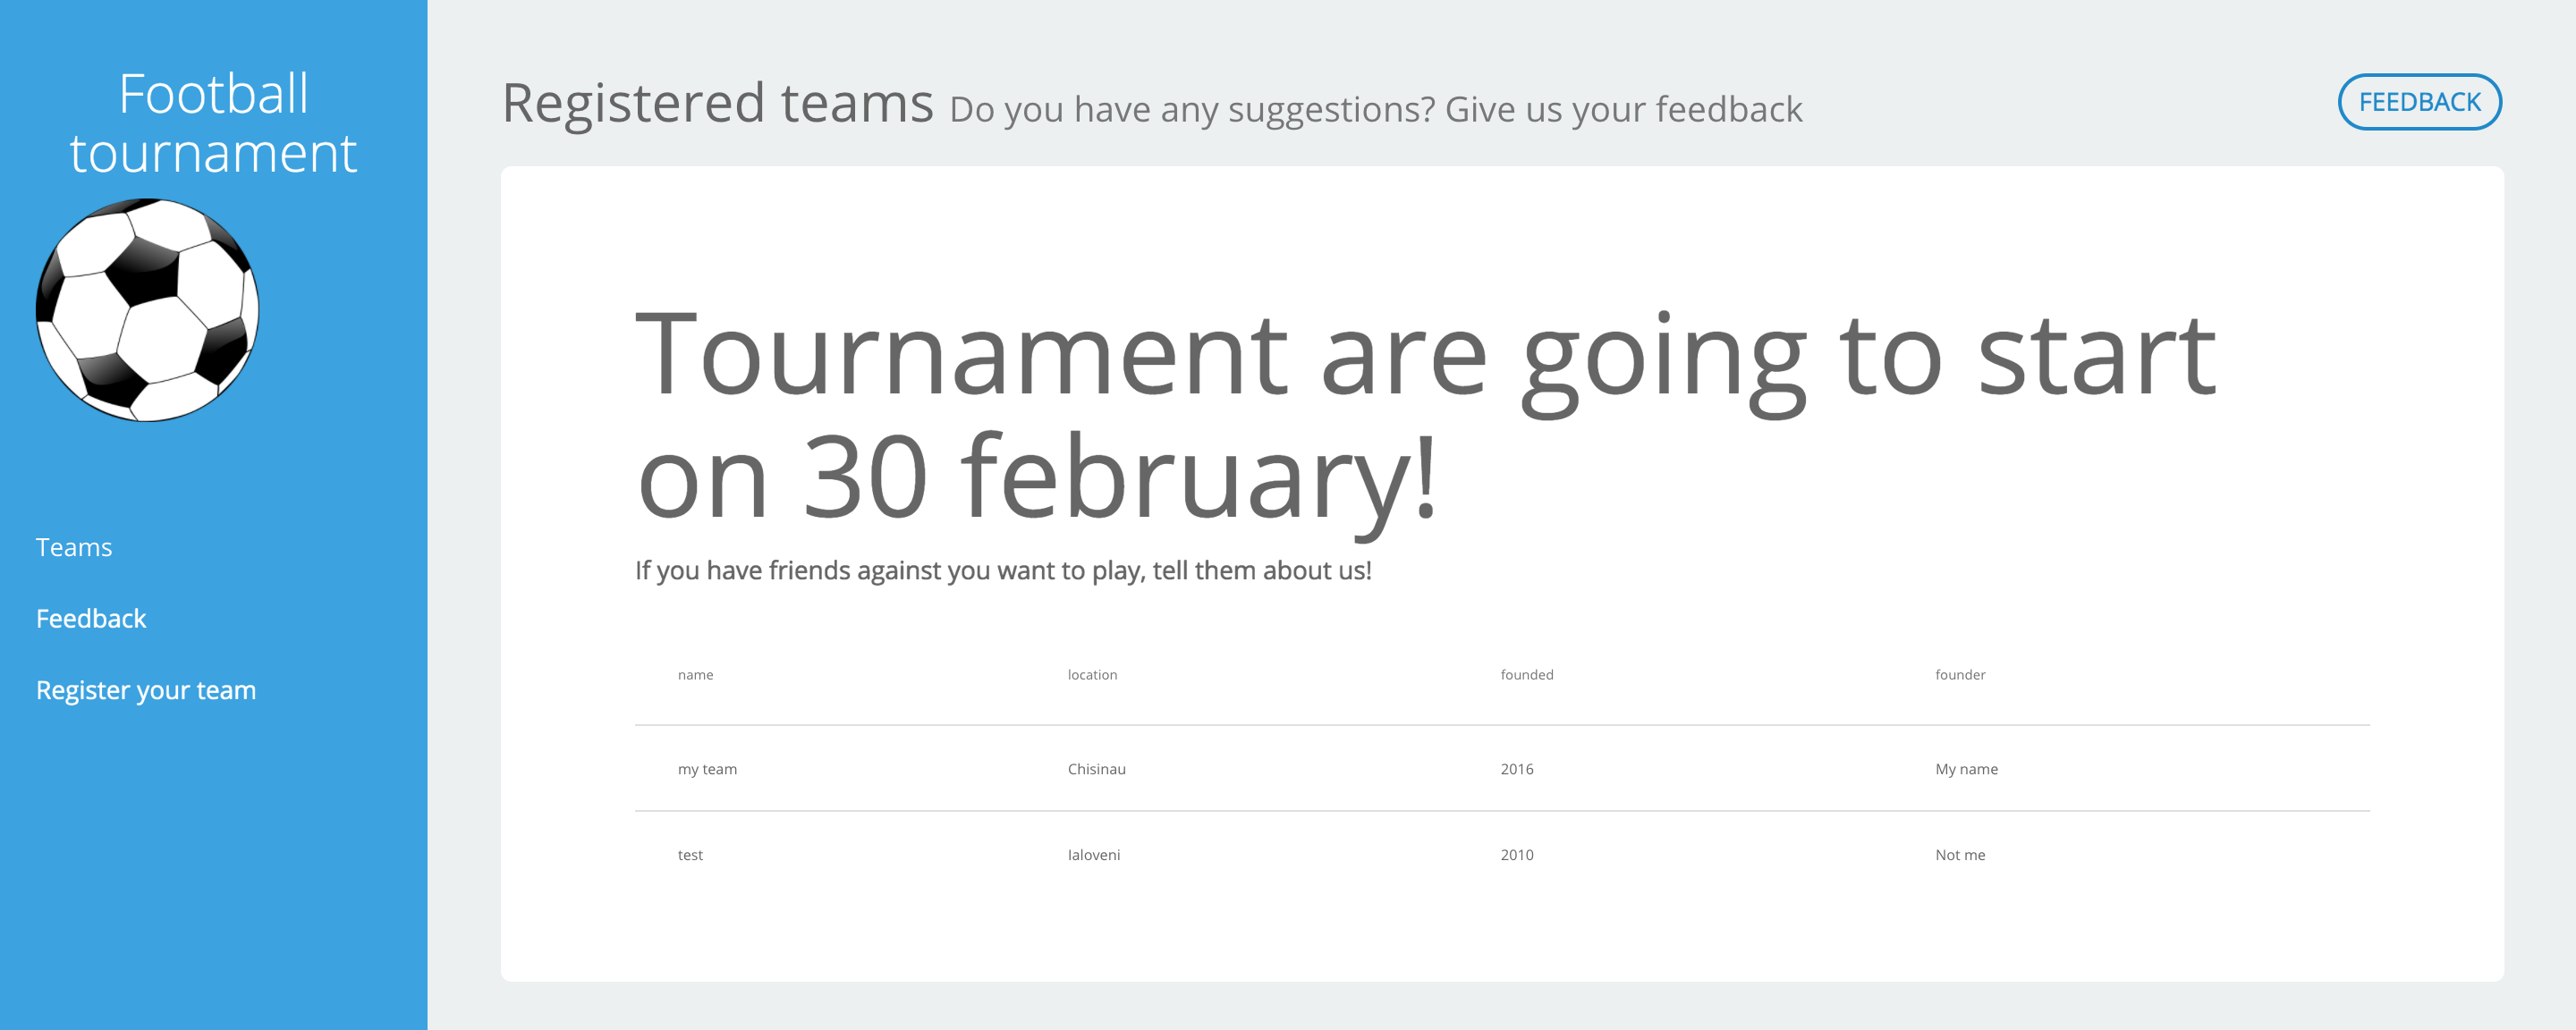
\includegraphics[width=15cm]{teams}\\
		\caption{Teams list}
		\label{run}
	\end{figure}
	
	\begin{figure}[h]
		\centering
		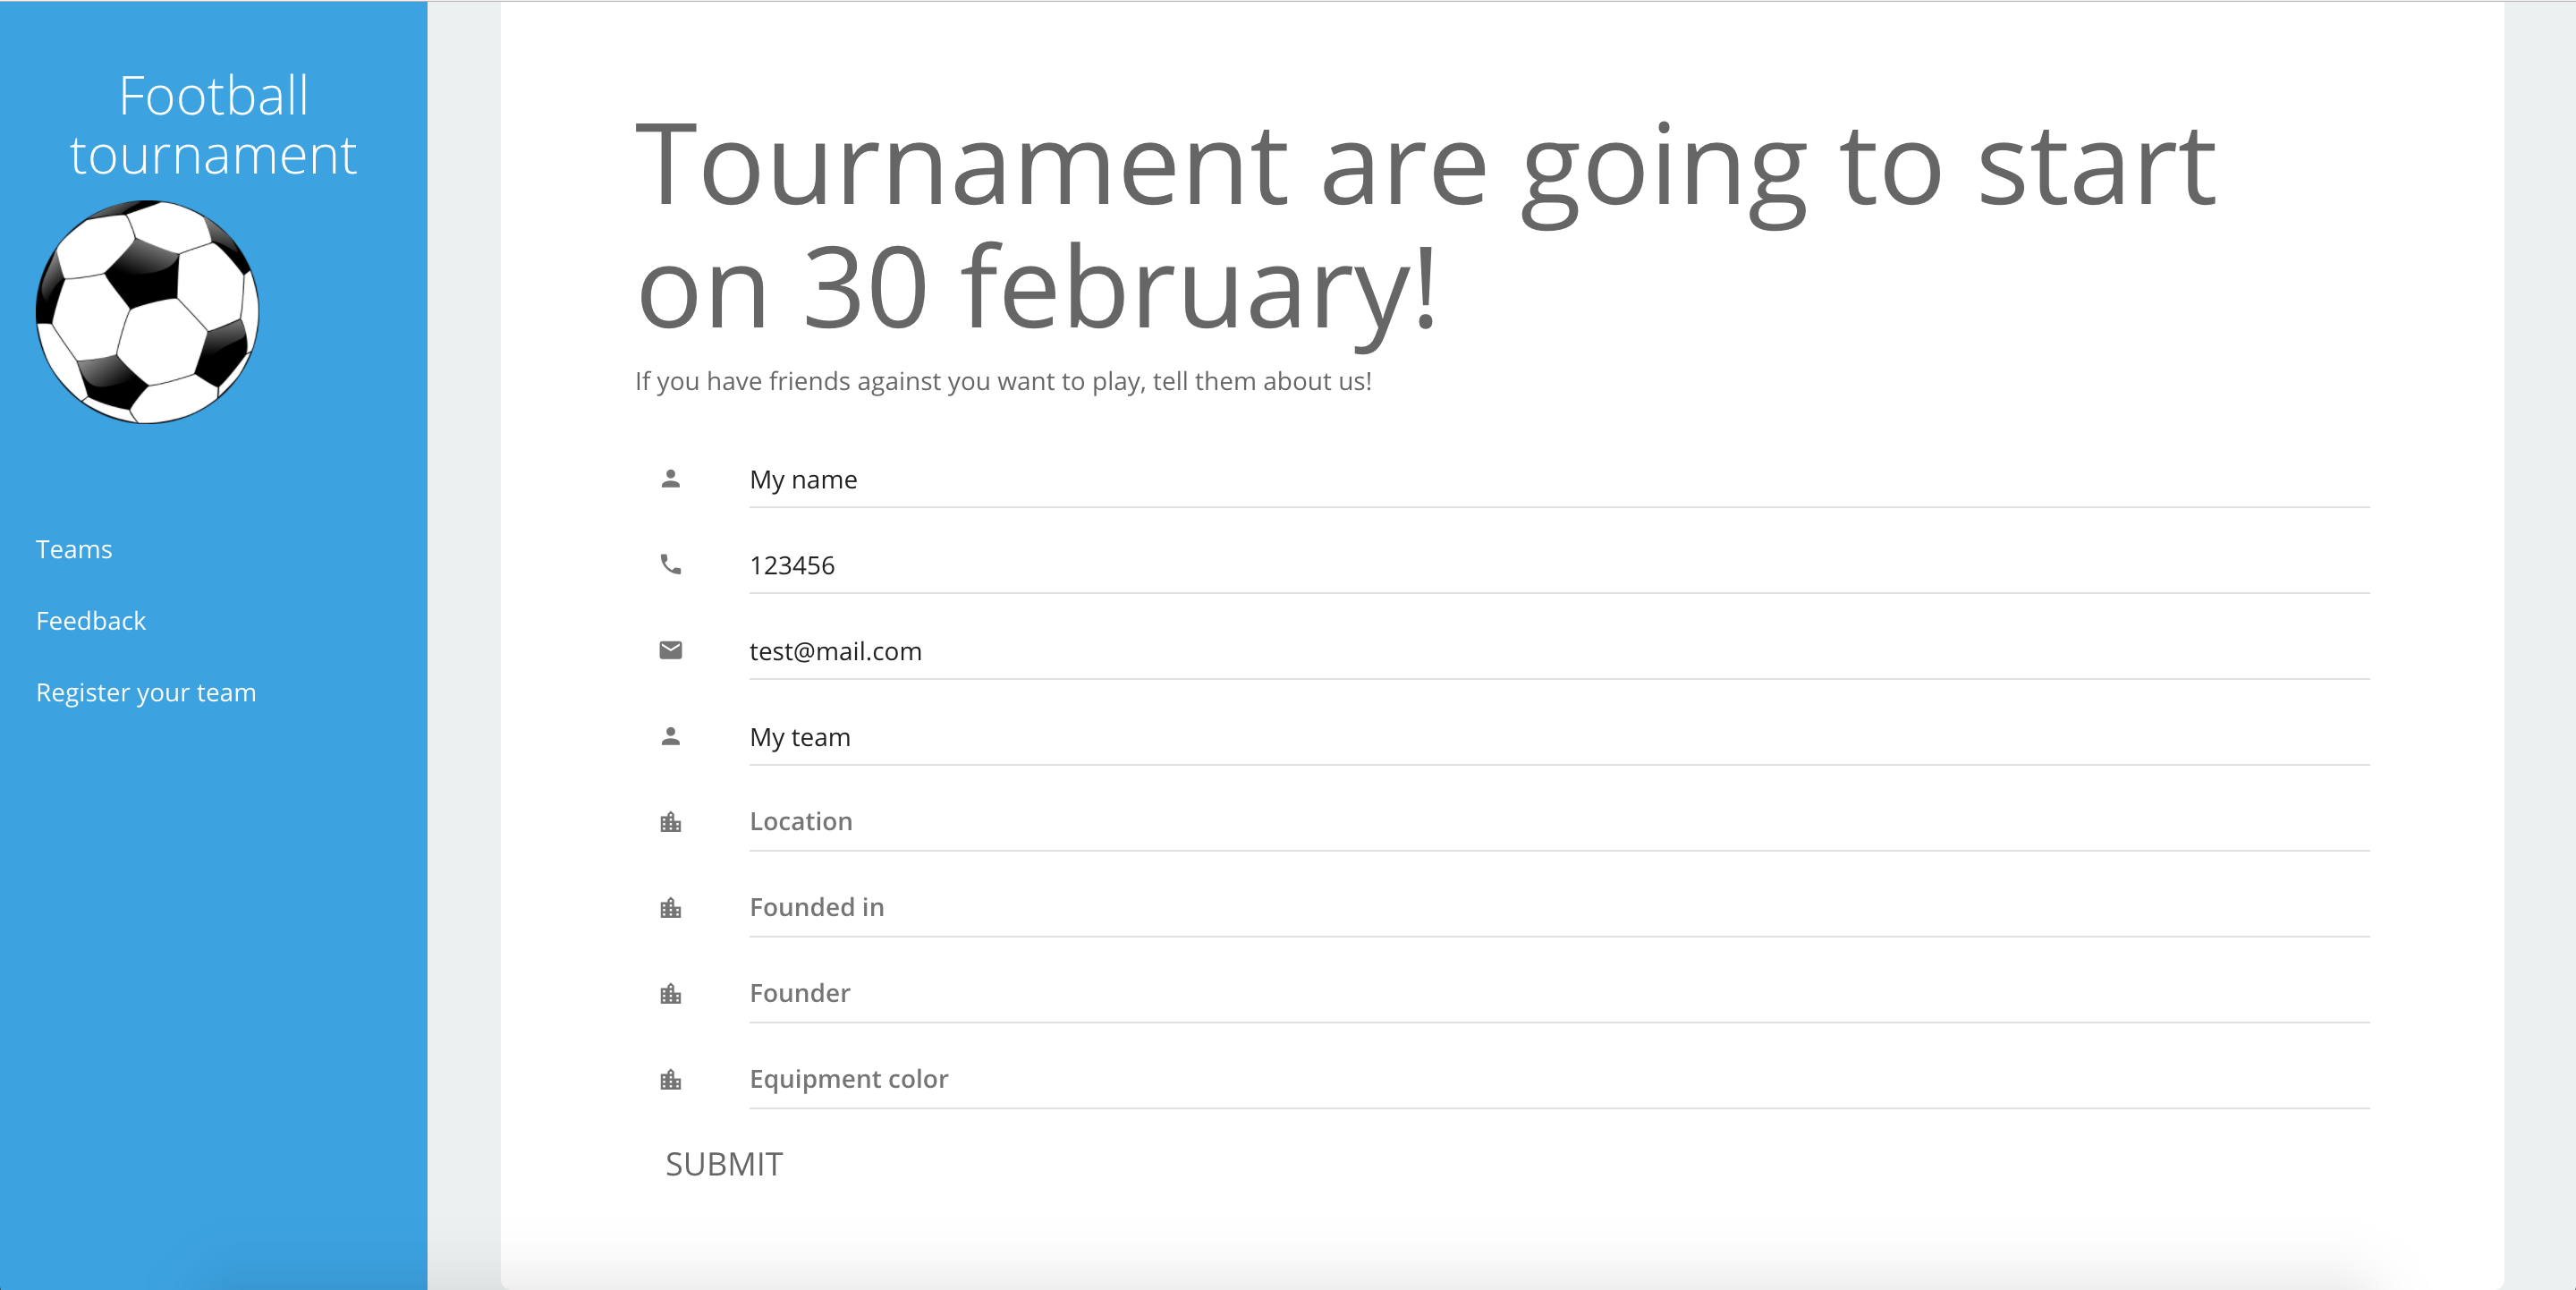
\includegraphics[width=15cm]{register}\\
		\caption{Register new team page}
		\label{jump}
	\end{figure}
	
	\begin{figure}[h]
		\centering
		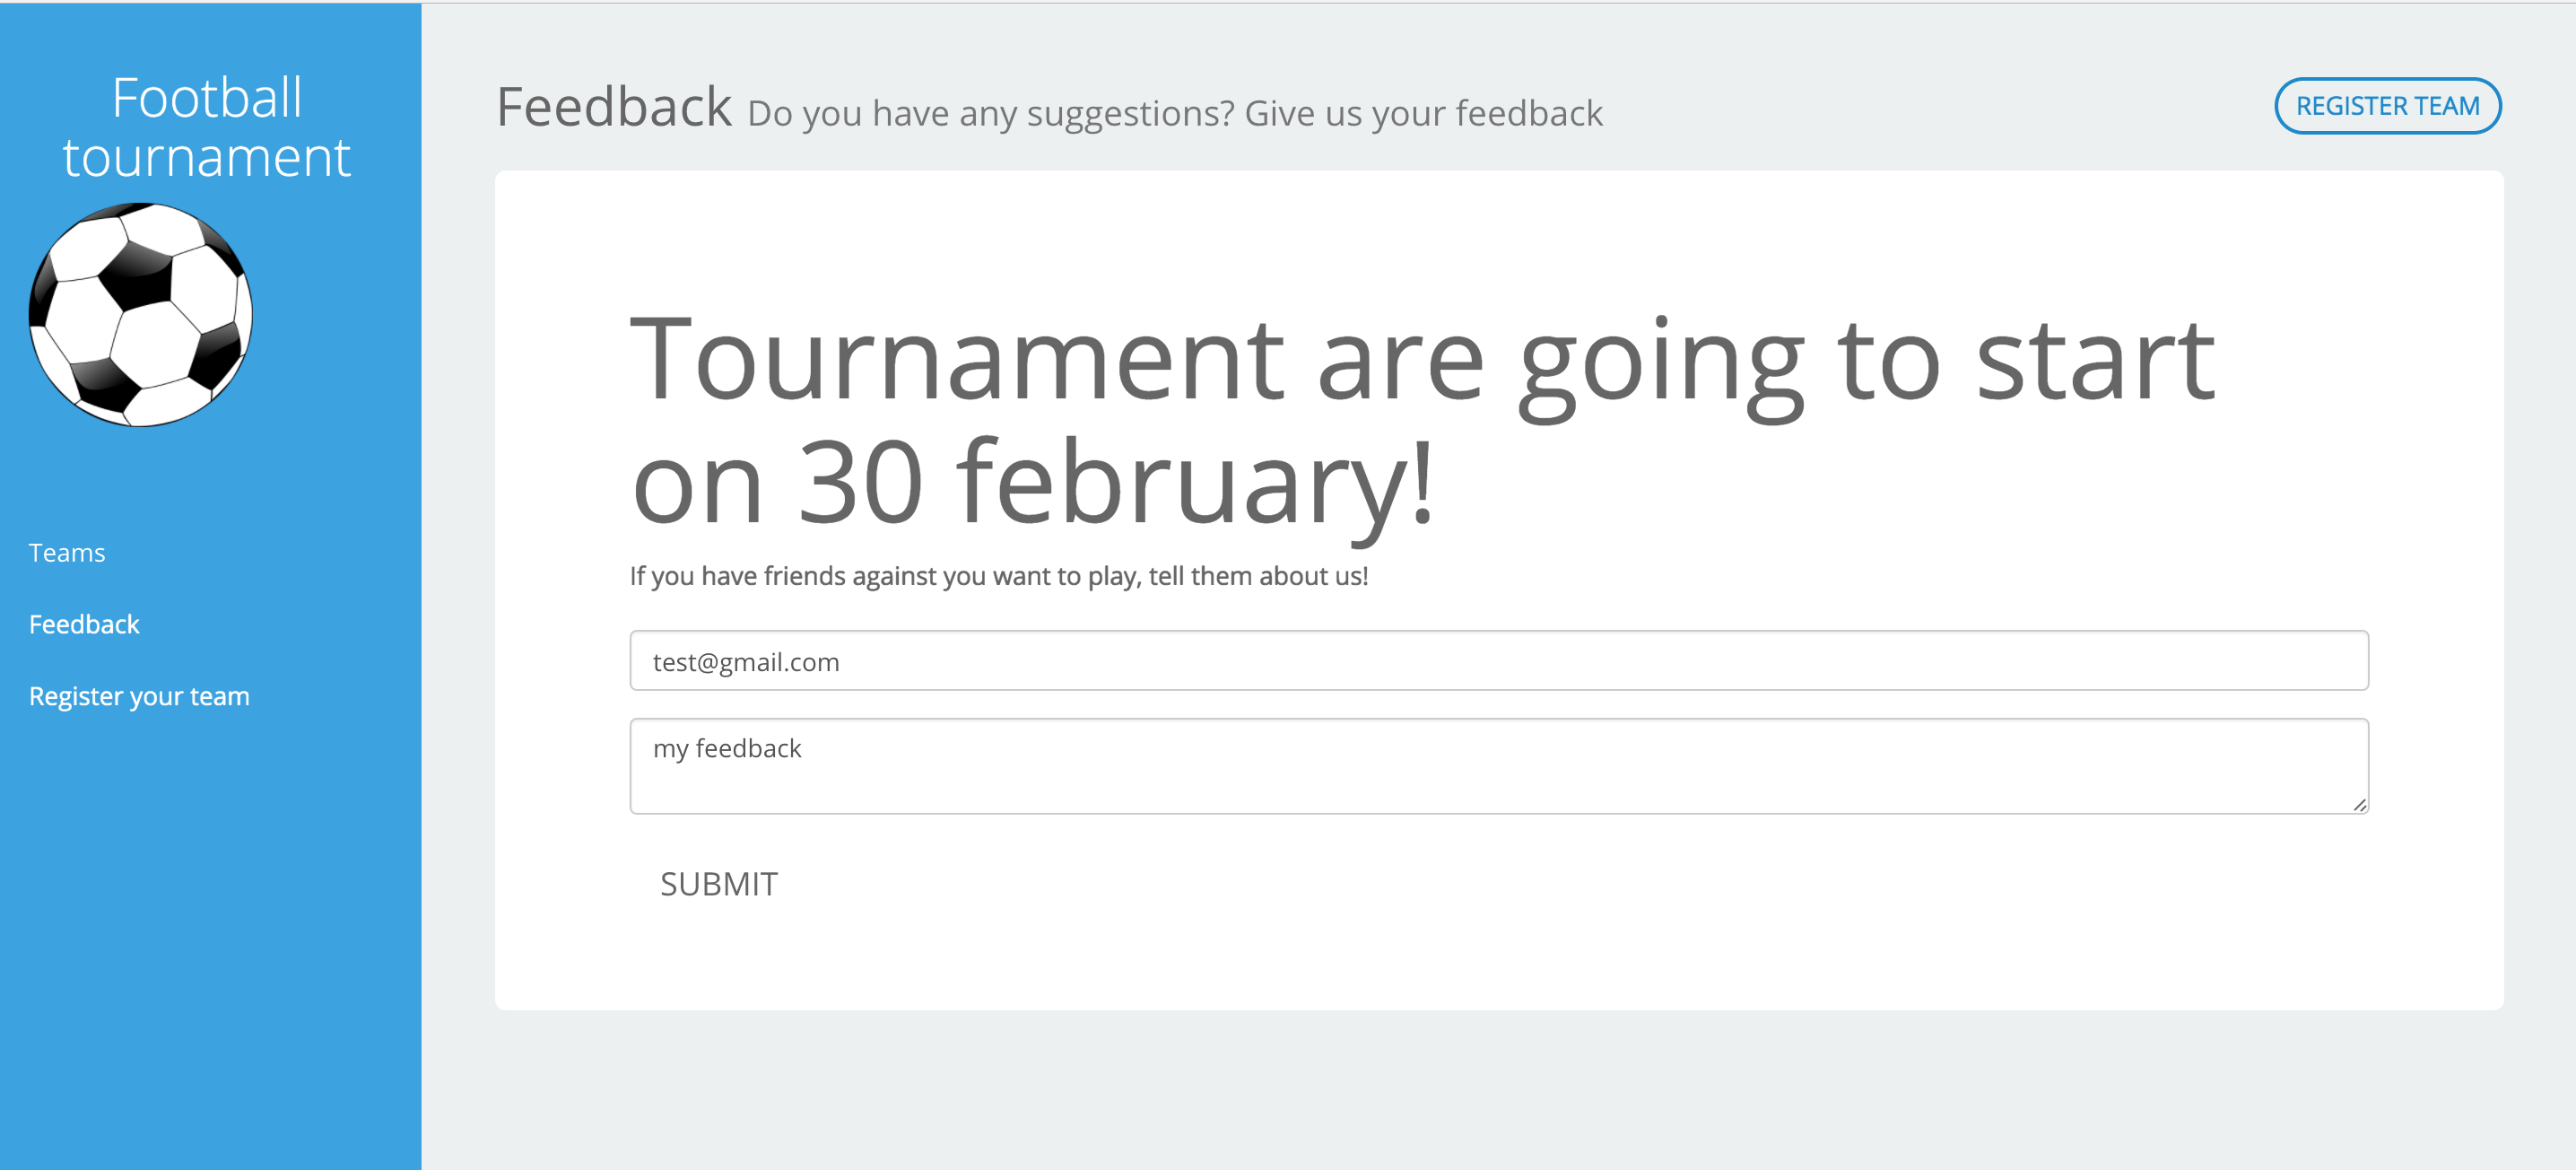
\includegraphics[width=15cm]{feedback}\\
		\caption{Feedback page}
		\label{slide}
	\end{figure}
	
	\begin{figure}[h]
		\centering
		
\includegraphics[width=10cm]{not-found}\\
		\caption{Not found page}
		\label{lose}
	\end{figure}
\end{center}

\clearpage